\section{Feature Representation Learning}
\label{feature-learning:sec}

The goal of this step is to learn to build the vector representations
for the nodes in the feature graphs at the method and statement levels.
At either level, the input includes the attributes of either a method
or a statement as in Figures~\ref{method-level-feature-extraction}
and~\ref{statement-level-feature-extraction}. The output is each
feature graph in which the nodes are replaced by their embeddings.

%In this step, \tool aims to learn the node feature embeddings based on the node features generated from step 1. So the input of this step is the method-level and statement-level graphs, and the expected output is the node embedding vectors for each node in each graph.

%To be more detailed, we also introduce the node feature representation learning from both method-level and statement-level.

\subsection{Method-level Representation Learning}

\begin{figure}[t]
	\centering
	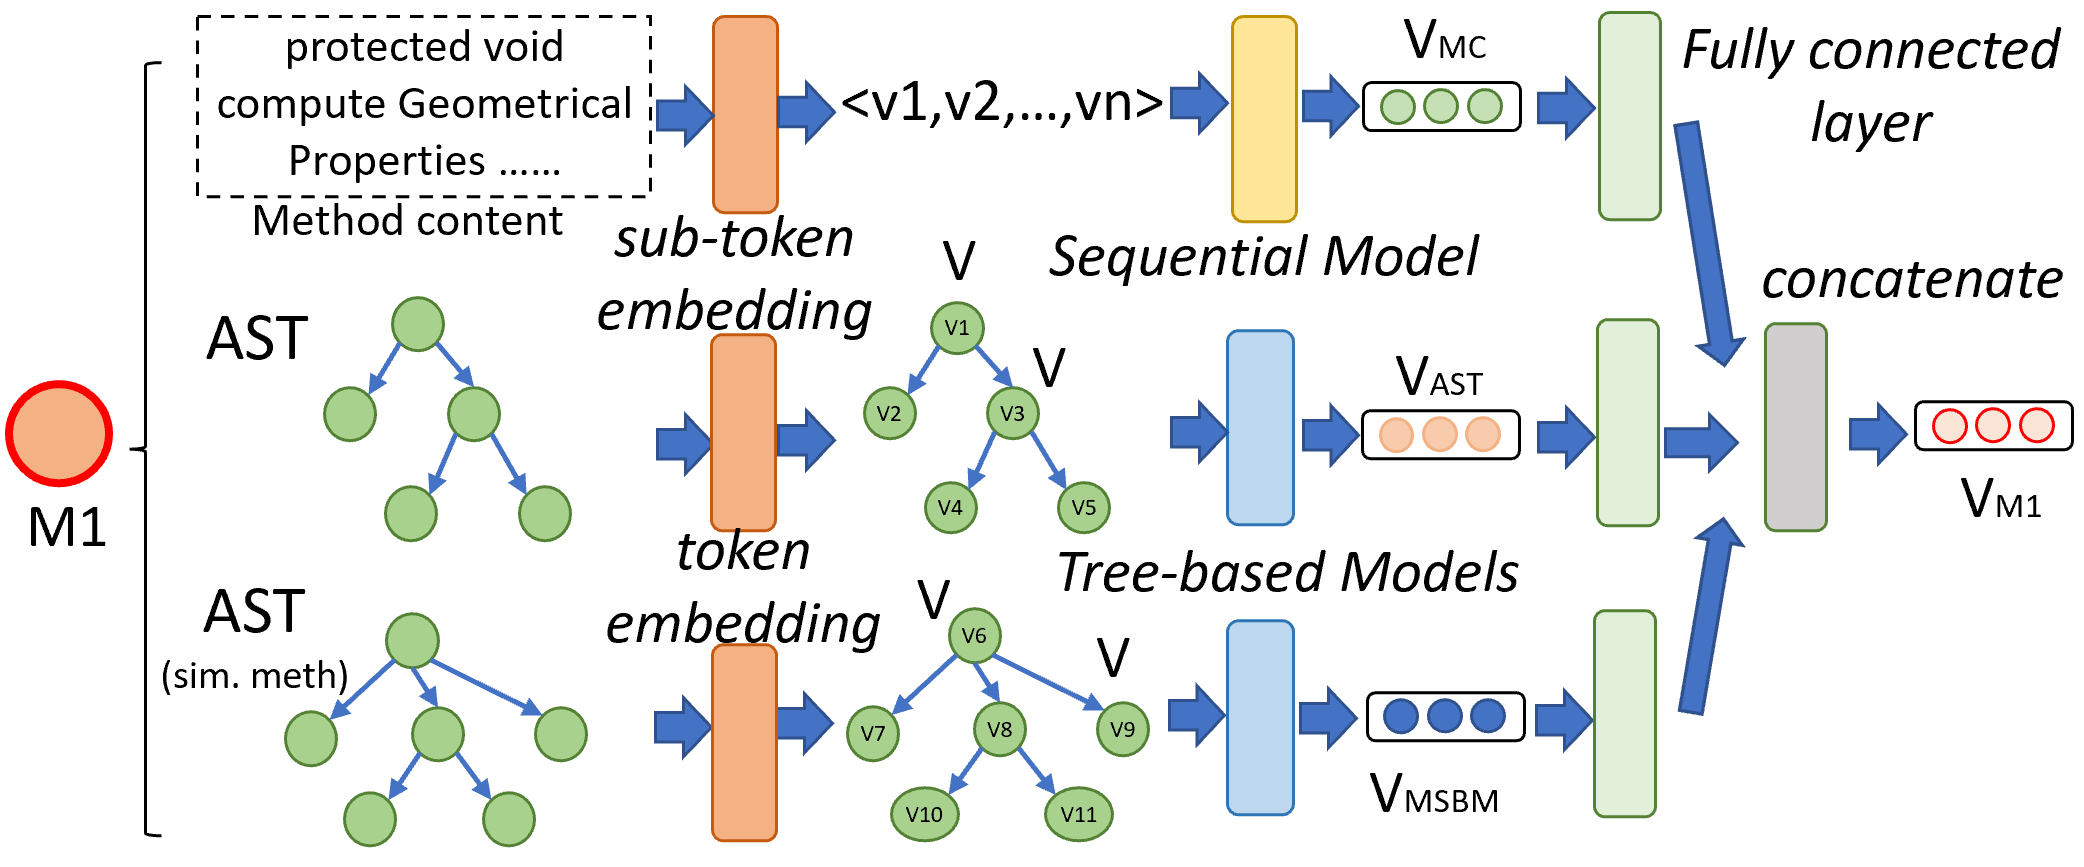
\includegraphics[width=3.4in]{graphs/step-2-method-new.png}
        \vspace{-14pt}
	\caption{Method-level Feature Representation Learning}
	\label{method-level-feature-learning}
\end{figure}

%From step 1, for each node representing a method $M$, there are extracted sequences of sub-tokens $Seq^p_m$ as the method content, generated AST $Tree_m$, and the generated AST for the most similar buggy method $M_b$ as the node features. Thus, to learn the feature representation, we follow these steps.

We process the attributes of a method as follows.

1) {\em \underline{The method's content}}: the method's content is
represented by the sequence $Seq_c$ of the sub-tokens built from the
code tokens in the interface and the body of the method. To vectorize
each sub-token in $Seq_c$ for representation, we use a word embedding
model, called GloVe~\cite{glove2014} to run on $Seq_c$. After this
vectorization, for the method, we obtain the sequence $<$ $v_1, v_2,
..., v_n$$>$ of the vectors of the sub-tokens in $Seq_c$.  We then
apply a sequential model on the sequence $<$$v_1,v_2,...,v_n$$>$ to learn
the ``summarized'' vector $V_{MC}$ that represents the method's
content. Specifically, we use Gated Recurrent Unit
(GRU)~\cite{cho2014learning}, a type of RNN layer that is efficient in
learning and capturing the information in the sequence.

%1) {\em \underline{The method's content}}: \tool uses the token embedding techniques to learn the representation vector for each token in the sequence and then replace each sub-token with the embedding vector generated from the techniques. The GloVe \cite{pennington2014glove} is a good word embedding technique that can catch the meaning of the sub-token well, so \tool uses GloVe as the token embedding technique. After the vectorization, \tool has a sequence of vector $Seq^{pe}_m$ and then uses a sequential model to learn the summarized vector that can represent the method's content.  GRU layer \cite{cho2014learning} is a type of RNN layer that is efficient in learning and summarizing the information in the sequences. \tool uses the GRU layer here to learn the embedding vector $V_{mc}$ for the method content. For example, as you can see in Figure \ref{method-level-feature-learning}, the method content first goes through the sub-token embedding bar and become a sequence of vectors. Each vector inside represents a sub-token. Such as $V_{geometrical}$ represent the sub-token $geometrical$. And then, this sequence is feed into the sequential model and gets the $V_{mc}$ as a summary to represent the method content.

2) {\em \underline{The method's structure}}: we first treat the
method as the sequence of tokens and use GloVe to build
the embeddings for all the tokens as in 1). We then replace every node
in the AST of the method with the GloVe's vector of the corresponding
token of the node (Figure~\ref{method-level-feature-learning}).  From
the tree of vectors, we use a tree-based model, called
TreeCaps~\cite{bui2021treecaps}, to capture its structure to
produce the ``summarized'' vector $V_{AST}$ representing the
method's structure.

%Similarly, \tool firstly uses the GloVe to vectorize the AST just as in 1) and then uses a tree-based model to learn the method's structure. One of the most recent studies, TreeCaps \cite{bui2021treecaps} proves that it is good at learning the tree structure information. So \tool uses TreeCaps as the tree-based model to learn the embedding vector $V_{AST}$ to catch the tree structure information. As shown in Figure \ref{method-level-feature-learning}, the generated AST firstly has been vectorized with GloVe and then use the tree-based model to get the representation vector $V_{AST}$

3) {\em \underline{Most similar faulty method}}: for each method, we
keep the most similar buggy one $M_b$. We process $M_b$ in the same
way as the method's structure via GloVe and TreeCaps to learn the
embedding vector $V_{MSBM}$ to represent $M_b$.

%As for the similar buggy method, \tool doing the same process as the method structure feature by using the GloVe and TreeCaps to learn the embedding vector $V_{MSBM}$. Similar as feature 2), in figure \ref{method-level-feature-learning}, the bottom line shows how the vector $V_{MSBM}$ generated for method $M1$

\subsection{Statement-level Representation Learning}

\begin{figure}[t]
	\centering
	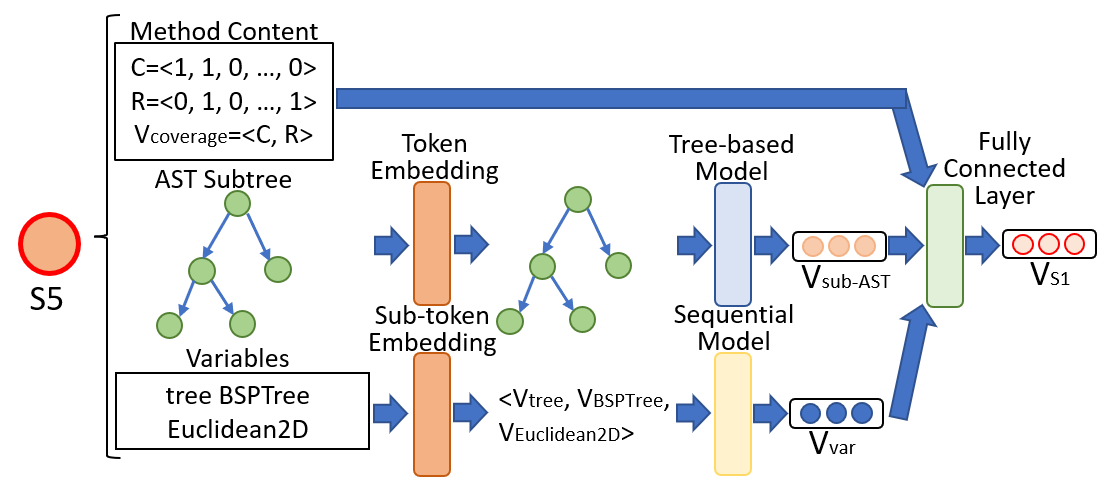
\includegraphics[width=3.4in]{graphs/step-2-statement-new.png}
        \vspace{-16pt}
	\caption{Statement-level Feature Representation Learning}
	\label{statement-level-feature-learning}
\end{figure}

We process the following attributes of a statement as follows.

1) {\em \underline{Code Coverage}}: we directly use the vector
$V_{Coverage} = <c_1, c_2, ...$, $c_K, r_1, r_2, ..., r_K>$ computed
from step 1 for the next computation.

%\tool does not make any changes and directly regard $V_{Cov} = <c_1,
%c_2, ..., c_K, r_1, r_2, ..., r_K>$ that is extracted from step 1 as
%the embedding vector $V_{cc}$ for the code coverage.

%From step 1, for each node representing a statement $S$, there are extracted code coverage information vector, generated AST subtree $Tree_s$, and the generated variable sequence as the node features. Thus, to learn the feature representation, we follow these steps.



2) {\em \underline{The statement's structure}}: we process the AST
subtree representing the statement's structure in the same manner (via
GloVe and TreeCaps) as for the method's structure to produce
$V_{subtree}$.


%\tool does the same process as the method's structure feature. \tool firstly using the GloVe to vectorize the AST and then using tree-based model TreeCaps to learn the embedding vector $V^{subtree}$. Just like the process steps for the AST subtree feature in Figure \ref{statement-level-feature-learning}.

3) {\em \underline{List of variables}}: we process this feature in the same
manner as the method's content (a sequence of sub-tokens). That is, we
apply the embedding model, GloVe, on the sequence of sub-tokens to
produce a sequence of vectors and then use a sequential model, GRU, to
produce the summarized vector for the list of variables.

%As for the similar buggy method, \tool doing the same process as the method structure feature by using the GloVe and TreeCaps to learn the embedding vector $V^{var}$. For example, in Figure \ref{statement-level-feature-learning}, the variable sequence $tree BSPTree Euclidean2D$ in $S5$ has been embedded through the sub-token embedding technique into $<V_{tree}, V_{BSPTree}, V_{Euclidean2D}>$ and then the sequential model learns the representation vector $V_{var}$ for the variable sequence. 

After computing the six embeddings for six attributes of a method and
a statement, we use six fully connected layers to standardize each
vector's length to $l/3$ (Here, l/3 is an integer). For a
method/statement, we concatenate the three output vectors from the
fully connected layer to produce the vector $V_{M}$ for the method or
$V_{S}$ for the statement with the length of $l$. After this 
step, we have the feature graph $G_{M}$ for each method and the graph
$G_{S}$ for each statement in which each node in each graph is
represented by a vector $V_{M}$ for a method or $V_{S}$ for a
statement computed as explained.

%After having the six embedding vectors mentioned above, \tool uses six fully connected layers to standardize each embedding vector's length to $l/3$ (Here l/3 is an integer). And then, for both method-level and statement-level, \tool concatenate three feature embedding vector into one vector $V_{M}$ or $V_{S}$ for the method-level or statement-level with the length of $l$. In this case, for both method-level and statement-level, \tool all has the graph $G_m$ or $G_s$ with the node embedding vector $V_{m}$ or $V_{s}$. It is the input for the next step.
